\chapter{Implementation and Results}
\label{chap:implementation-and-results}

Simulating and solving for the same parameters, we can compare the radial distribution histogram of the simulation output with the obtained, radially symmetric, equilibrium distribution $\rho \in \functionspace$, cf. \Cref{fig:simulation-solver-comparison}.

% describe how we find the minimum potential and export in C++

\begin{figure}[H]
  \centering
  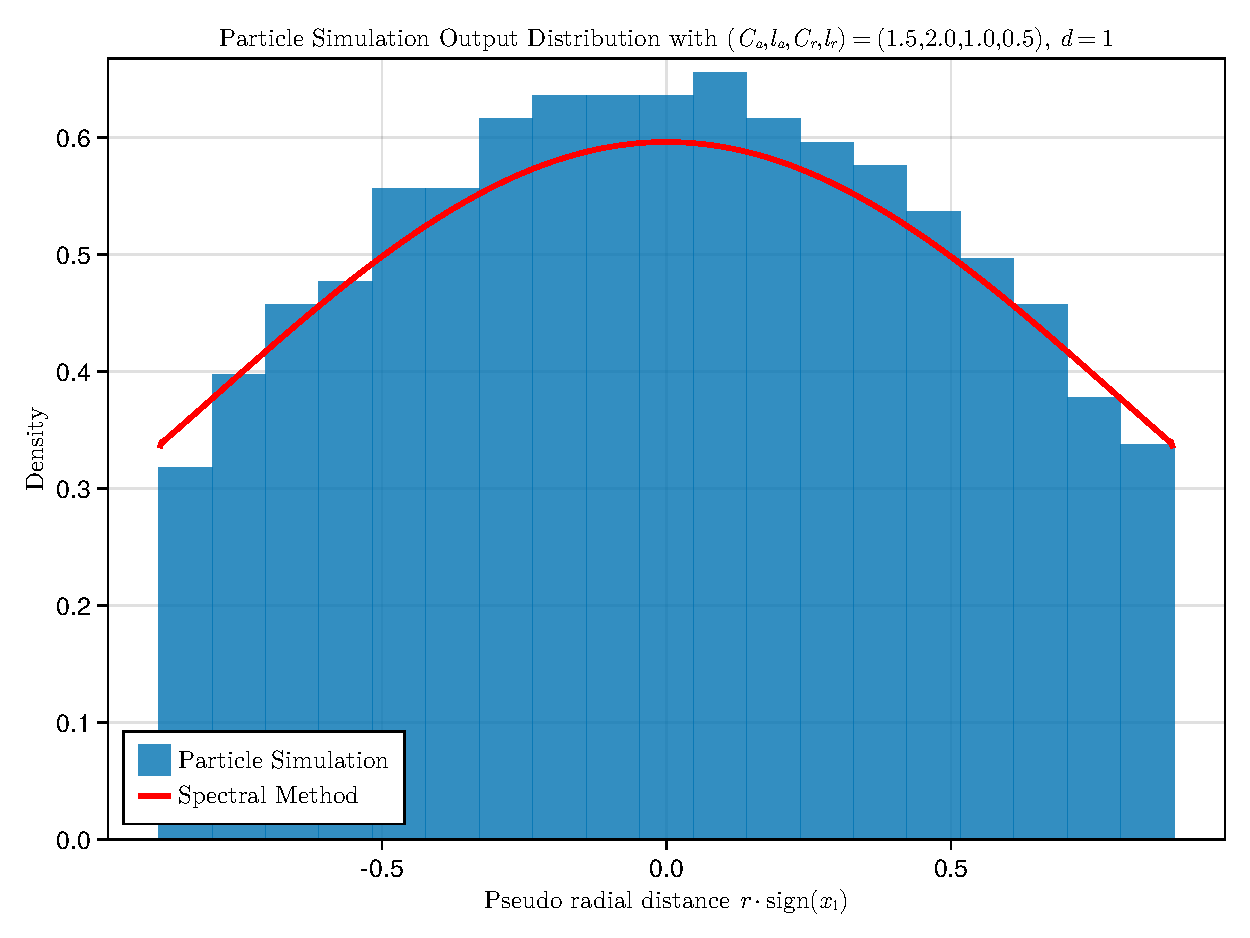
\includegraphics[width=0.8\linewidth]{results/morse/simulation-solver-comparison.pdf}
  \caption[Comparison of histogram and spectral method solution]{Comparison of the radial distance histogram from the simulation output with the $G = 8$ general kernel solver's equilibrium measure $\rho_{12}(r)$ at $R$ given by the simulator, so without using the outer optimisation routine. The interaction potential in this example is $K(r) = K_{C_a, l_a, C_r, l_r}(r)$ with parameters given above.}
  \label{fig:simulation-solver-comparison}
  % for now
\end{figure}

\section{Further Discussion}
\subsection{Well-Conditionedness}
A common flaw of spectral (collocation) methods, one could think of them as the highest-order limit of finite difference schemes, is their problematic conditioning behaviour, often caused by to the ill-conditioning of spectral differentiation matrices \parencite{2019-atap}.

Ideally, we would like the condition number $\kappa_2(Q) \in \R$ to be independent of the order $N$ to which we solve our problem.
For well-conditionedness of the operator, we need
$$\kappa_2(Q) := \frac{\sigma_{\rm max}(Q)}{\sigma_{\rm min}(Q)} = \frac{\norm{Q}}{\norm{Q^{-1}}} = \mathcal{O}(1)\,,$$
and not $\mathcal{O}(N)$ or even higher orders.
The poor conditioning behaviour of the operators in the attractive-repulsive case can be seen in \Cref{fig:condition-number-growth}.
Attempts at using a preconditioner similar to the proposal in \cite{2013-a-fast-and-well-conditioned-spectral-method} to improve the conditioning to $\kappa_2(Q) = \mathcal{O}(1)$ were unsuccessful.

\begin{figure}[H]
  \centering
  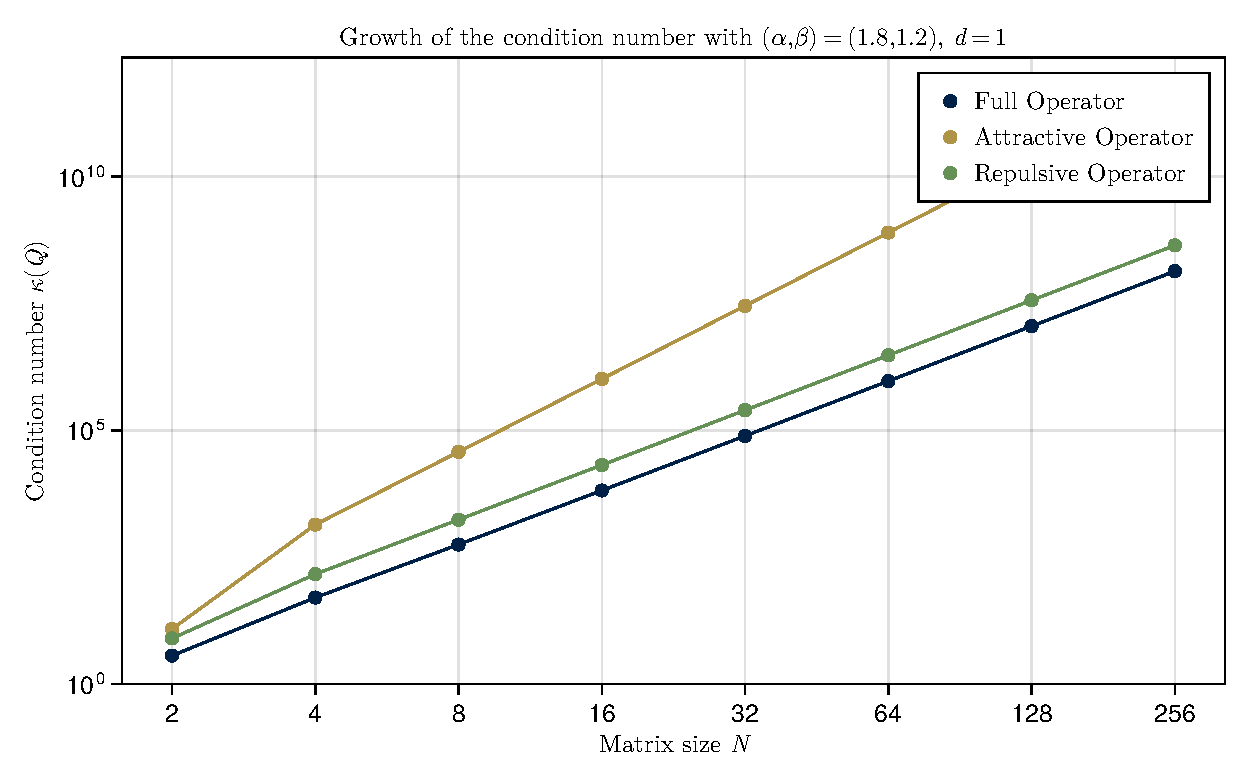
\includegraphics[width=0.8\linewidth]{results/attrep/condition-number-growth.pdf}
  \caption[Growth of the condition number]{Growth of the 2-norm condition number $\kappa_2(Q)$ of the attractive-repulsive operators $Q^{(\alpha)}$, $Q^{(\beta)}$ and $Q_{\alpha,\beta}$ for growing system size $N$.}
  \label{fig:condition-number-growth}
\end{figure}

The improvement of coefficient decay for high orders $N$ due to Tikhonov regularisation, as discussed in \Cref{sec:regularisation}, can be seen in \Cref{fig:coefficients}.

\begin{figure}[H]
  \centering
  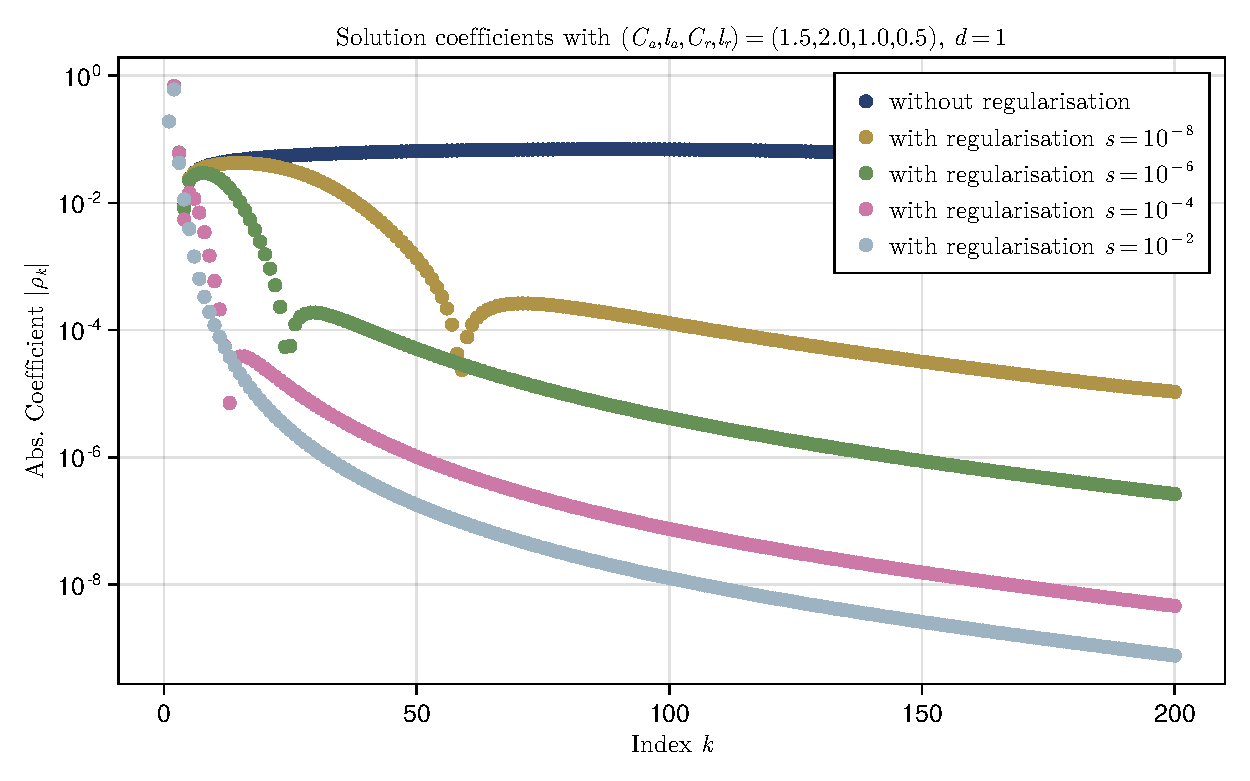
\includegraphics[width=0.75\linewidth]{results/morse/coefficients.pdf}
  \caption[Absolute value of the coefficients with and without regularisation]{Absolute value of the solution coefficients $\rho_k$ with and without Tikhonov regularisation after the solution of a $200 \times 200$ linear system.}
  \label{fig:coefficients}
\end{figure}

\section{Implementation Architecture}
The spectral method solver is written in Julia \parencite{2017-julia} whereas the simulator is written in C++.
To compile the simulator, please run \\
\bashblock{mkdir build; cd build/; cmake .. -DCMAKE\_BUILD\_TYPE=Release} \\
\bashblock{make -j4}
in a bash terminal.

In order to run tests of the numerical solver implementation, run \\
\bashblock{julia solver/tests.jl} \\
in a bash terminal. In order to regenerate all plots at once, including simulation output from the C++ implementation, run \\
\bashblock{julia solver/plotall.jl} \\
in a terminal.
More details can be found in the code repository \parencite{2023-my-dissertation}.

In the attractive-repulsive case, the full solution process, including the construction of the operator and solving a linear system, takes \SI{2.68 \pm 0.02}{\milli\second} with a memory allocation estimate of around \SI{2}{\mega\byte}, for an operator of size $N=30$ (enough for most real-world applications).
For an operator of size $N = 200$, it takes \SI{850 \pm 20}{\milli\second} with a memory estimate of about \SI{500}{\mega\beta}.
In the case of the general kernel spectral method, the solution takes \SI{3.24 \pm 0.03}{\milli\second} for $N=30$.
For $N=200$, it takes \SI{970 \pm 36}{\milli\second}.
Both require a similar amount of memory as in the attractive-repulsive case.
These benchmarks were accumulated on an Intel \textregistered \, i7-5600U CPU running at \SI{2.6}{\giga\hertz}, as the average over 50 individual runs.
